\documentclass[a4paper,10pt]{article}
%\documentclass{svjour3}
\usepackage{a4wide}
\usepackage[utf8]{inputenc}
\usepackage[T1]{fontenc}

%\usepackage{tcolorbox}
\usepackage{subcaption}
\usepackage{amsmath,amssymb}
\usepackage{amsthm}
%\usepackage{calrsfs} % nice cal fonts
\usepackage{enumerate} 
%\usepackage[toc,page]{appendix}

%\usepackage[auth-sc]{authblk}
\usepackage{authblk}
\renewcommand\Affilfont{\normalfont\small}

\usepackage[round]{natbib}
\bibliographystyle{spbasic}
\bibpunct[, ]{(}{)}{;}{a}{}{,}
\let\bibfont\relax
\def\bibfont{\fontsize{8}{10}\selectfont}
\setlength{\bibsep}{0pt}

\usepackage[svgnames]{xcolor}
\usepackage[pdftex]{hyperref}
\hypersetup{
    colorlinks=true,
    colorlinks,
    linkcolor=Navy,
    citecolor=Navy,
    urlcolor=Navy
}
%\definecolor{highlightNEW}{named}{Navy} %To get all equation in black:
\definecolor{highlightNEW}{named}{black}

\usepackage{graphicx}
\graphicspath{{fig/}}
\usepackage{epstopdf}
\usepackage{booktabs}
\usepackage{multirow}

% custom macros and definitions
\newtheorem{theorem}{Theorem}[section] 
%%\newtheorem{acknowledgement}[theorem]{Acknowledgement} 
%%\newtheorem{algorithm}[theorem]{Algorithm} 
%%\newtheorem{axiom}[theorem]{Axiom} 
%%\newtheorem{case}[theorem]{Case} 
%%\newtheorem{claim}[theorem]{Claim} 
%%\newtheorem{conclusion}[theorem]{Conclusion} 
%%\newtheorem{condition}[theorem]{Condition} 
%%\newtheorem{conjecture}[theorem]{Conjecture}
\newtheorem{definition}[theorem]{Definition}
\newtheorem{corollary}[theorem]{Corollary} 
%%\newtheorem{criterion}[theorem]{Criterion} 
%%\newtheorem{defi}[theorem]{Definition} 
\newtheorem{example}[theorem]{Example} 
%%\newtheorem{exercise}[theorem]{Exercise} 
\newtheorem{hypothesis}[theorem]{Hypothesis} 
\newtheorem{lemma}[theorem]{Lemma} 
%%\newtheorem{notation}[theorem]{Notation} 
%%\newtheorem{problem}[theorem]{Problem} 
\newtheorem{proposition}[theorem]{Proposition} 
%%\newtheorem{question}[theorem]{Question} 
\newtheorem{remark}[theorem]{Remark} 
%%\newtheorem{solution}[theorem]{Solution} 
%%\newtheorem{summary}[theorem]{Summary} 
%%\newtheorem{Rem}[theorem]{Remark}

\newcommand{\TODO}[1]{\textbf{\color{red}TODO: {#1}}\PackageWarning{TODO:}{#1!}}
\newcommand{\doi}[1]{DOI~\href{\detokenize{http://dx.doi.org/#1}}{\detokenize{#1}}}

\renewcommand{\d}{\,\mathrm{d}}
\newcommand{\e}{\mathrm{e}}
\newcommand{\E}{\mathbb{E}}
\newcommand{\F}{\mathcal{F}}
\renewcommand{\H}{\mathcal{H}}
\newcommand{\K}{\mathfrak{K}}
\newcommand{\N}{\mathbb{N}}
\renewcommand{\P}{\mathbb{P}}
\newcommand{\R}{\mathbb{R}}
\newcommand{\Var}{\mathbb{V}ar}
\newcommand{\1}{\mathbf{1}}

\newcommand{\la}{\!\left\langle}
\newcommand{\ra}{\right\rangle}
\newcommand{\p}{\partial}

%\newcommand*{\Cdot}{\raisebox{-0.25ex}{\scalebox{1.2}{\ensuremath{\cdot}}}}
\newcommand*{\Cdot}[1][1.25]{%
  \mathpalette{\CdotAux{#1}}\cdot%
}
\newdimen\CdotAxis
\newcommand*{\CdotAux}[3]{%
  {%
    \settoheight\CdotAxis{$#2\vcenter{}$}%
    \sbox0{%
      \raisebox\CdotAxis{%
        \scalebox{#1}{%
          \raisebox{-\CdotAxis}{%
            $\mathsurround=0pt #2#3$%
          }%
        }%
      }%
    }%
    % Remove depth that arises from scaling.
    \dp0=0pt %
    % Decrease scaled height.
    \sbox2{$#2\bullet$}%
    \ifdim\ht2<\ht0 %
      \ht0=\ht2 %
    \fi
    % Use the same width as the original \cdot.
    \sbox2{$\mathsurround=0pt #2#3$}%
    \hbox to \wd2{\hss\usebox{0}\hss}%
  }%
}
\makeatletter
\def\mathcolor#1#{\@mathcolor{#1}}
\def\@mathcolor#1#2#3{%
  \protect\leavevmode
  \begingroup
    \color#1{#2}#3%
  \endgroup
}
\makeatother


\newcommand{\NEW}[1]{\mathcolor{highlightNEW}{#1}}
\let\oldalpha\alpha
\renewcommand{\alpha}{\mathcolor{highlightNEW}{\oldalpha}}
\newcommand{\ccode}[2]{\par
        \vspace*{8pt}
        {{\leftskip18pt\rightskip\leftskip
        \noindent{\it #1}\/: #2\par}}\par}
\newcommand{\keywords}[1]{\ccode{Keywords}{#1}}
\newcommand{\email}[1]{\href{mailto:#1}{#1}}

\title{\textcolor{Navy}{\textsc{Convexity adjustments with a bit of Malliavin}}}

\author[1,2]{David Garcia-Lorite\thanks{Corresponding author, \email{dddd@caixabank.es}}}
\author[3]{Ra\'{u}l Merino}

\affil[1]{CaixaBank, Quantitative Analyst Team, Plaza de Castilla, 3, 28046 Madrid, Spain,}
\affil[2]{Facultat de Matem\`{a}tiques i Inform\`{a}tica, Universitat de Barcelona, \authorcr Gran Via 585, 08007 Barcelona, Spain,\vspace*{3pt}}
\affil[3]{VidaCaixa S.A., Market Risk Management Unit, \authorcr C/Juan Gris, 2-8, 08014 Barcelona, Spain.}

%\date{Received: date / Accepted: date}
\date{\normalfont\small\today}

% main document
\begin{document}

\maketitle
\begin{abstract}
AA
\end{abstract}
%\keywords{V--}
%\ccode{MSC classification}{--}
%\ccode{JEL classification}{--}

%\TODO{Remove ToC in final version}
%\tableofcontents
%\clearpage

\section{Introduction}
Mathematical finance aims to find a methodology to price consistently all the instruments quoted in the market. When working with fixed income derivatives, a classic research topic is the introduction of a price adjustment to achieve this. This adjustment is called convexity adjustment. It is non-linear and depends on the interest rate model.  

There are several reasons to include this type of adjustment. One of them is to incorporate futures on the yield curve construction. Futures and other fixed-income instruments are quoted differently. The firsts are linear against the yield, but the others are not. Therefore, the changes in value and yield of different contracts are different. This difference will depend on the volatility and correlation of the yield curve.

But it is not the only one. The fixed-income market has several features changing the schedule of payments. For example, in a swap in arrears, the floating coupon fixing and payment are on the same date. Or in a CMS swap, the floating rate is linked to a rate longer than the floating length. Any customization of an interest rate product based on changing time, currency, margin, or collateral will require a convexity adjustment. Deep down, by making these changes, we are mixing the martingale measures. 

Convexity adjustments have become popular again. Not only by the increase in volatility in the markets. In addition, as a consequence of the transition in risk-free rates from the IBOR (InterBank Offered Rates) indices to the ARR (Alternative Reference Rates) indices, also called RFR. Both indices try to represent the same thing, the risk-free rate, but they are fundamentally different. While the former represents the average rate at which Panel Banks believe they could borrow money, the latter is calculated backward based on transactions. Therefore, these new products need their corresponding convexity adjustment. 

The first references on the convexity adjustment were \cite{RitchkenS}, \cite{Flesaker} and \cite{BrothertonIben}, published almost simultaneously. A convexity formula for averaging contracts was found in \cite{RitchkenS}. Flesaker derived a convexity adjustment for computing the expected Libor rate under the Ho-Lee model in a continuous and discrete setting in \cite{Flesaker}. \cite{BrothertonIben} used the Taylor expansion on the inverse function for calculating the convexity adjustment. In the following years, several improvements were made. For example, the convexity adjustment was extended to other payoffs in \cite{Hull06}. \cite{Hart} improved the Taylor expansion. \cite{KirikosNovak} derived the convexity adjustment for the Hull-White model. Afterwards, we can find papers that extend the convexity adjustment to different payoffs, see \cite{Benhamou00WC} or \cite{Hagan03}. Or by applying alternative techniques such as the change of measure in \cite{Pelsser}, a martingale approach in \cite{Benhamou00} or the effects of stochastic volatility in \cite{PiterbargRenedo} and \cite{HaganWoodward20}.

In the present paper, we find an alternative way to calculate the convexity adjustment for a general interest rate model. The idea is to use the It\^o's representation theorem. Unfortunately, the theorem does not give an insight into how to calculate the elements therein. Therefore, it is necessary to introduce basic concepts of Malliavin calculus to apply the Clark-Ocone representation formula.

The structure of the paper is as follows. In Section \ref{sec:Notation}, we give the basic preliminaries and our notation related to Interest Rates models. This notation will be used throughout the paper without being repeated in particular theorems unless we find it useful to do so in order to guide the reader through the results. In Section \ref{sec:Malliavin}, we make an introduction to Malliavin calculus. In Section \ref{sec:CA}, we compute the convexity adjsustment for several payoffs that are presents as usual way in the interest rate trading desks. As well, we do some numerical expresents to check the analytical results obtained. To end, in Section \ref{sec:Conclusion} we give the conclusions of the paper and future lines of research to explore.


\section{Preliminaries and notation}\label{sec:Notation}
Consider a continuous-time economy where zero-coupon bonds are traded for all maturities. The price at time $t$ of a zero-coupon bond with maturity $T$ is denoted by $P(t,T)$ where $0\leq t \leq T$. Clearly, $P(T,T)=1$. We define the compounded instantaneous forward rate forward rate as:
\begin{eqnarray*}
f(t,T)= -\partial_{T}\ln P(t,T)
\end{eqnarray*}
and the spot interest rates as:
\begin{eqnarray*}
r(t)=\lim_{T\longrightarrow t} -\partial_{T}\ln P(t,T).
\end{eqnarray*}
We have that the price of a zero-coupon bond is given by
\begin{eqnarray*}
P(t,T)=\exp\left(-\int^{T}_{t} f(t,u) du\right).
\end{eqnarray*}

Before the financial crisis, there was a single curve framework where there was a single curve for discounting and forecasting. Since then, the market has adopted a multi-curve approach with two different curves: the discounting curve and the estimation curve chosen based on the maturity of the underlying rate. The difference between these two curves is known as basis. In this paper, we will assume that the basis are not stochastic. Therefore can be directly obtained from the market at time $t=0$. In other words, the estimation forward curve $f_{E}(t, T)$ is given by
\begin{equation}\label{estimation_forward_rate_curve}
f_{E}(t,T) = f_{ois}(t,T) + s(t,T)
\end{equation}
where and $f_{ois}$ is the discount curve and $s(t,T)$ are the basis between the two curves, i.e. $s(t,T)= f_{E}(0,T) - f_{ois}(0,T)$.\\

We will assume that the $f_{ois}$ dynamics follows a single factor Heath-Jarrow-Morton model under the $\mathbb{Q}$-measure. Therefore, let $T>0$ a fixed time horizon, $t>0$ the starting time, and $W$ a Brownian motion defined on a complete probability space $(\omega, \mathcal{F}, \mathbb{P})$. Then, under the HJM we have the following dynamics
\begin{align}\label{ois_forward_rate_curve}
df_{ois}(t,T) &= \sigma(t,T)\nu(t,T)dt + \sigma(t,T)dW^{\mathbb{Q}}_t
\end{align}
where $\nu(t,T)=\int_{t}^{T}\sigma(t,s)ds$ and $\sigma(t, T)$ are $\mathcal{F}_{t}$-adapted process that are positive functions for all $t,T$ . In particular, we have that
\begin{eqnarray*}
f_{ois}(t,T)= -\partial_{T}\ln P_{ois}(t,T).
\end{eqnarray*}

In order to have a Markovian representation of the HJM, we will assume that the volatility is separable, i.e.
\begin{equation}
\sigma(t,T)= h(t)g(T).
\end{equation}
with $g$ a positive time-dependent function and $h$ a non-negative process. In addition
\begin{align*}
\eta_t &= g(t)h(t,x_t,y_t)  \nonumber \\
k_t &= - \frac{\partial_t g(t)}{g(t)}.
\end{align*}
Throught this paper, we assume the following hypotheses on $\eta(t,x,y)$.
\begin{hypothesis}\label{boundedness_volatility} 
The process $\eta_t$ is global Lipschitz and differentiable a.s. In addition, we will suppose that
\begin{align*}
\alpha_1 \leq \eta(t,x,y) \leq \alpha_2 \quad \forall (t,x,y) \in \mathbb{R}^{+} \times \mathbb{R} \times \mathbb{R}^{+}. \\
|\eta(t,x_2,y_2) - \eta(t,x_1,y_1)| \leq C_{x,y} \lVert (x_2-x_1,y_2-y_1)\rVert \quad \forall (t,x,y) \in \mathbb{R}^{+} \times \mathbb{R} \times \mathbb{R}^{+} 
\end{align*}
with $\lVert \cdot \rVert$ euclidean norm in $\mathbb{R}^{2}$.
\end{hypothesis}
\begin{hypothesis}\label{boundedness_reversion} 
The mean reversion function $k(\cdot)$ is a continuous and positive a.s such that
\begin{equation*}
m_k < k(t) \leq M_k \quad \forall t \geq 0.
\end{equation*}

\begin{remark}
Under these assumptions on $k(\cdot)$, we have that
\begin{equation*}
\lim_{t \to \infty}  I(\alpha,0,t):= \lim_{t \to \infty} \int_{0}^{t} \exp\left(-\alpha \int_{u}^{t} k(s) ds\right) du \leq \frac{1}{\alpha m_k} \quad \text{with} \quad \alpha > 0.
\end{equation*}
On other hand, as well it is easy to show that
\begin{equation*}
\lim_{t \to \infty}  J(\alpha,0,t):= \lim_{t \to \infty} \int_{0}^{t} G^{\alpha}(u,t) \exp\left(-\alpha \int_{u}^{t} k(s) ds\right) du \leq \frac{1}{\alpha m^{\alpha+1}_{k}}
\end{equation*}
\end{remark}

\end{hypothesis}
\begin{remark}
Notice that the above hypotheses have been chosen for the sake of simplicity, but they can be replaced by adequate integrability conditions.
\end{remark}
We must note, that under the hypothesis (\ref{boundedness_volatility}) $\partial_x \eta(t,x,y)$ and $\partial_y \eta(t,x,y)$ are bounded. This version of the HJM is also known as the Cheyette model, \cite{Cheyette}. It is easy to show (see \cite{Andreasen01} that
\begin{equation}
r_{ois}(t)=f_{ois}(t,t)= f_{ois}(0,t) + x_t,
\end{equation}  
where
\begin{align}\label{short_rate_cheyette}
dx_t &= (-k_t x_t + y_t)dt + \eta(t,x_t,y_t) dW_t^{\mathbb{Q}} \nonumber \\
dy_t &= (\eta^{2}_t - 2 k_t y_t) dt ,
\end{align} 
with 
\begin{align*}
\eta_t &= g(t)h(t,x_t,y_t)  \nonumber \\
k_t &= - \frac{\partial_t g(t)}{g(t)}.
\end{align*}
Now if we do a little bit of algebra and we use Itô formula we can show the next representation formula for $P_{ois}(t,T)$
\begin{equation}\label{bond_ois}
P_{ois}(t,T) = \frac{P_{ois}(0,T)}{P_{ois}(0,t)} \exp\left(-G(t,T)x_t - \frac{1}{2} G^{2}(t,T)y_t \right)
\end{equation}
where $G(t,T) = \int_{t}^{T} \exp\left(-\int_{t}^{u} k_s ds \right) du$. We must observe, that under the representation (\ref{estimation_forward_rate_curve}) we have that
\begin{equation}\label{bond_forward}
P_{E}(t,T)=H(t,T)P_{ois}(t,T)
\end{equation}
where $H(t,T)=\exp\left(-\int_{t}^{T}s(t,u) du \right)$.

\section{Basic introduction to Malliavin calculus}\label{sec:Malliavin}
Malliavin calculus is an infinite-dimensional calculus in a Gaussian space, that is, a stochastic calculus of variations. In other words, this is a theory that provides a way to calculate the derivatives of random variables defined in a Gaussian probability space with respect to the underlying noise. The initial objective of Malliavin was the study of the existence of densities of Wiener functionals such as solutions of stochastic differential equations. But, nowadays, it has become an important tool in stochastic analysis due to the increase in its applications. Some of these applications include stochastic calculus for fractional Brownian motion, central limit theorems for multiple stochastic integrals, and an extension of the Itô formula for anticipative processes, but especially mathematical finance. For example, we can apply Mallaivin calculus for computing hedging strategies, Greeks, or obtain price approximations. See, for example, \cite{AlosLorite} or \cite{Nualart} for more general content.\\

In our case, we are interested in using the Malliavin calculus to apply the Clark–Ocone representation theorem. But, first of all, let's introduce some basic concepts.\\ 

Now, we introduce the derivative operator in the Malliavin calculus sense and the divergence operator to establish the notation that we use in the remainder of the paper.\\

Consider $W=\left\{W_{t}, t\in \left[0,T\right]\right\}$ a Brownian motion defined on a complete probability space $\left(\Omega, \mathcal{F}, \mathbb{P}\right)$. Let $H=L^{2}(\left[0,T\right])$ and denote by 
\begin{eqnarray*}
W_{t} := \int^{T}_{0} t_{s} \d W_{s},
\end{eqnarray*}
the It\^o integral of a deterministic function $h \in H$, also known as Wiener integral. Let $\mathcal{S}$ be the set of smooth random variables of the form
\begin{eqnarray*}
F=f\left(W_{t_{1}}, \ldots, W{t_{n}}\right)
\end{eqnarray*}
with $t_{1}, \ldots, t_{n} \in \left[0,T\right]$ and $f$ is infinitely differentiable bounded function.

\medbreak

The derivative of a random variable $F$, $D_{s}F$, is defined as the stochastic process given by
\begin{eqnarray*}
D_{s}F = \sum^{n}_{i=1} \frac{\partial f}{\partial x_{i}}\left(W_{t_{1}}, \ldots, W_{t_{n}}\right)1_{\left[0, t_{j}\right]}(s), \hspace{0.4cm} s \in \left[0,T\right].
\end{eqnarray*}

The iterated derivative operator of a random variable $F$ is defined by
\begin{eqnarray*}
D^{m}_{s_{1}, \ldots, s_{m}} F = D_{s_{1}} \cdots D_{s_{m}}F, \hspace{0.4cm} s_{1}, \ldots, s_{m} \in \left[0,T\right].
\end{eqnarray*}

\cite{Nualart} stated that these operators are closable from $L^{p}(\Omega)$ into $L^{p}(\Omega; L^{2}\left[0,T\right])$ for any $p\geq1$, and we denote by $\mathbb{D}^{n,p}$ the closure of $\mathcal{S}$ with respect to the norm
\begin{eqnarray*}
\left\|F\right\|_{n,p} := \left(E\left[F\right]^{p} + \sum^{n}_{i=1} E\left\|D^{i} F\right\|^{p}_{L^{2}\left(\left[0,T\right]^{i}\right)} \right)^{\frac{1}{p}}.
\end{eqnarray*}

\medbreak 

We define $\delta$ as the adjoint of derivative operator $D$, also referred to as the Skorohod integral. The domain of $\delta$, denoted by $Dom\text{ }\delta$, is the set of elements $u \in L^{2}([0,T] \times \Omega)$ such that there exists $\delta(u) \in L^{2}(\Omega)$ satisfying the duality relation
\begin{eqnarray*}
E\left[\delta(u) F \right] = E\left[\int^{T}_{0} \left(D_{s} F\right) u_{s} \d s\right].
\end{eqnarray*}

The operator $\delta$ is an extension of the Itô integral in the sense that the set $L^{2}_{a}([0,T] \times \Omega)$ of square integrable and adapted processes is included in $Dom\text{ }\delta$ and the operator $\delta$ restricted to $L^{2}_{a}([0,T] \times \Omega)$ coincides with the Itô stochastic integral.

\medbreak

For any $u \in Dom\text{ }\delta$, we will use the following notation
\begin{eqnarray*}
\delta(u)=\int^{T}_{0}u_{s}\d W_{s}.
\end{eqnarray*}

\medbreak

The representation of functionals of Brownian motion by stochastic integrals, also known as martingale representation, has been widely studied over the years. It states that if $F$ is a square-integrable random variable, there exists a unique adapted process $\varphi$ in $L^{2}(\Omega \times \left[0,T\right]; \mathbb{R}^{d})$ such that
\begin{eqnarray*}
F=E\left[F\right] + \sum^{n}_{i=1}\int^{T}_{0} \varphi^{i}_{s} dW^{i}_{s}.
\end{eqnarray*}
In other words, there exists a unique martingale representation or, more precisely, the integrand $\varphi$ in the representation exists and is unique in $L^{2}(\Omega \times \left[0,T\right]; \mathbb{R}^{d})$.

\medbreak

Unfortunately, it is not easy to find an analytic representation of the process $\varphi$. Here, the Malliavin calculus helps us to find a solution. When the random variable $F$ is Malliavin differentiable, the process $\varphi$ appearing in It\^o's representation theorem, is given by
\begin{eqnarray*}
\varphi^{i}=E\left[D^{W^{i}}_{t}F|\mathcal{F}^{W}_{s}\right].
\end{eqnarray*}
In fact,
\begin{eqnarray}\label{clark-okone}
F=E\left[F\right] + \sum^{n}_{i=1}\int^{T}_{0} E\left[D^{W^{i}}_{t}F|\mathcal{F}^{W}_{s}\right] dW^{i}_{s}
\end{eqnarray}
is the Clark-Ocone representation formula. 

 

\section{Convexity Adjustment}\label{sec:CA}
In this section, we derive the convexity adjustment for different products. The advantage of using the Malliavin calculus is that it allows us to derive a general representation formula . In order to introduce a general idea of the method. Let define a $Z_t = f(x_t)$. Now, we suppose that $Z_t$ is martingale under the measure $\mathbb{Q}_1$ and that we want to compute $\mathbb{E}^{\mathbb{Q}_2}\left(Z_T \right)$, where $\mathbb{Q}_2$ is a measure such that $dW^{\mathbb{Q}_1}_t = dW^{\mathbb{Q}_2}_t +\lambda_t dt$. Then, if we use the Clark-Ocone representation, we have that
\begin{equation*}
f(x_t) = \mathbb{E}^{\mathbb{Q}_1}\left(f(x_t)\right) + \int_{0}^{t} \mathbb{E}^{\mathbb{Q}_1}_s\left( f^{\prime}(x_t) D_s x_t  \right) dW^{\mathbb{Q}_1}_s
\end{equation*}
Now, if we take $\mathbb{E}^{\mathbb{Q}_2}\left( \cdot \right)$ in the previous expression and we use the Girsanov's theorem, we get that
\begin{equation}\label{general_convexity}
\mathbb{E}^{\mathbb{Q}_2}\left( f(x_t) \right) = f(x_0) + \mathbb{E}^{\mathbb{Q}_1} \left(\int_{0}^{t}  \mathbb{E}^{\mathbb{Q}_1}_s\left( f^{\prime}(x_t) D_s x_t  \right) \lambda_s ds \right). 
\end{equation}
The second term, is the convexity adjustment to due to change of measure from $\mathbb{Q}_1$ to $\mathbb{Q}_2$. The differents choice of $f$, $\mathbb{Q}_1$ and $\mathbb{Q}_2$ will allow us to get an approximation of the convexity adjustment for the different case of interest. 
\subsection{FRAs Vs futures}
 The cash flows in FRAs and futures are computed under different measures. Consequently, we need to adjust the futures price quote to transform them into FRAs price quotes. As usual, we will define the forward rate at time $t_0$ between $t_1$ and $t_2$ under the forward curve $E$ as:
\begin{equation}\label{forward_rate}
L_{E}(t_0, t_1, t_2) = \frac{\left(\frac{P_{E}(t_0,t_1)}{P_{E}(t_0,t_2)} - 1 \right)}{\delta_{t_1,t_2}}
\end{equation} 
where $P_{E}(t,T)$ is the discount factor for the curve $E$ from $t$ to $T$, and $\delta_{t_1,t_2}$ is the year fraction between $t_1$ and $t_2$. Observe that $L_{E}(t, t_1, t_2)$ is a martingale under the forward measure $\mathbb{Q}^{t_2}$. Let us define the future rate as:    
\begin{equation}\label{future}
\hat{L}_{E}(t,t_0, t_1, t_2) = \mathbb{E}_t^{\mathbb{Q}}\left(L_{E}(t_0, t_1, t_2) \right), 
\end{equation}
where $\mathbb{Q}$ is the measure associated to the numeraire $B_t=\exp\left(\int_{0}^{t} r_{ois, s} ds \right)$ with $ r_{ois, t}$ the risk free short rate. Using
\eqref{forward_rate} and \eqref{future}, then the convexity adjustment definition is:
\begin{equation*}
CA(t, t_0, t_1, t_2) = \hat{L}_{E}(t,t_0, t_1, t_2) - \mathbb{E}_t^{\mathbb{Q}^{t_2}}\left(L_{E}(t_0, t_1, t_2) \right).
\end{equation*}
From (\ref{ois_forward_rate_curve}) and since $f_{ois}(t,T)$ is a $\mathbb{Q}^{T}$ martingale, we have that
\begin{equation}\label{girsanov_spot_forward}
dW^{\mathbb{Q}^{t_2}} = dW^{\mathbb{Q}} + \nu(t,t_2) dt. 
\end{equation}
Now, if we use (\ref{general_convexity}) with $f(x_t)=L_{E}(t,t_0, t_1, t_2)$, $\mathbb{Q}_1=\mathbb{Q}$, $\mathbb{Q}_1=\mathbb{Q}^{t_2}$ and $\lambda_t = \nu(t,t_2)$,  we get that
\begin{equation}\label{ca_general_future}
CA(t, t_0, t_1, t_2) = \mathbb{E}^{\mathbb{Q}^{t2}}\left(\int_{0}^{t_0} \mathbb{E}^{\mathbb{Q}}_{s}\left(D_s L_{E}(t_0,t_1,t_2) \right) \nu(s,t_2) ds \right)
\end{equation}
where $\nu(t,T)$ has been defined in (\ref{ois_forward_rate_curve}). Now, from the definition of $L_{E}(t,T)$. Now, if we calculate the malliavin derive of $L_{E}(t_0,t_1,t_2)$ we have that
\begin{equation*}
D_s L_{E}(t_0,t_1,t_2) = \frac{H(t_0,t_1)}{\delta_{t_1,t_2}H(t_0,t_2)} D_s \left(\frac{P_{ois}(t_0,t_1)}{P_{ois}(t_0,t_2)}\right) 
\end{equation*}
Now from the zero coupon representation formula (\ref{bond_ois}) we get that
\begin{equation*}
D_s \left(\frac{P_{ois}(t_0,t_1)}{P_{ois}(t_0,t_2)}\right) = \frac{\left(\partial_{x}P_{ois}(t_0,t_1)P_{ois}(t_0,t_2) - \partial_{x}P_{ois}(t_0,t_2) P_{ois}(t_0,t_1) \right)}{P^{2}_{ois}(t_0,t_2)} D_s x_{t_0}
\end{equation*}
therefore
\begin{equation}\label{malliavin_derive_L}
D_s L_{E}(t_0,t_1,t_2) = \frac{H(t_0,t_1)}{\delta_{t_1,t_2}H(t_0,t_2)}\frac{\left(\partial_{x}P_{ois}(t_0,t_1)P_{ois}(t_0,t_2) - \partial_{x}P_{ois}(t_0,t_2) P_{ois}(t_0,t_1) \right)}{P^{2}_{ois}(t_0,t_2)} D_s x_{t_0} 
\end{equation}
If we use (\ref{approximation_D_s_x_t}) with $T_a=t_0$ and $\beta(t,t_0,x,y) = \exp\left(-\int_{s}^{T_a}k_u du \right) \eta(u,x,y)$ we have that
\begin{align*}
D_s L_{E}(t_0,t_1,t_2) &\approx \frac{H(t_0,t_1)}{\delta_{t_1,t_2}H(t_0,t_2)}\frac{\left(\partial_{x}P_{ois}(t_0,t_1)P_{ois}(t_0,t_2) - \partial_{x}P_{ois}(t_0,t_2) P_{ois}(t_0,t_1) \right)}{P^{2}_{ois}(t_0,t_2)} \beta(t,t_0,\bar{x}_s,\bar{y}_s)\bar{M}(s,t_0) \nonumber \\
\approx& \frac{P_{E}(0,t_1)}{\delta_{t_1,t_2} P_{E}(0,t_2)} \left(G(t_0,t_2) \frac{P_{ois}(0,t_2)}{P_{ois}(0,t_0)} - G(t_0,t_1) \frac{P_{ois}(0,t_1)}{P_{ois}(0,t_0)} \right)\beta(t,t_0,\bar{x}_s,\bar{y}_s)\bar{M}(s,t_0)
\end{align*}
and therefore
\begin{equation}\label{approximation_clarkocone}
\mathbb{E}_s\left( D_s L_{E}(t_0,t_1,t_2) \right) = \frac{P_{E}(0,t_1)}{\delta_{t_1,t_2} P_{E}(0,t_2)} \left(G(t_0,t_2)  - G(t_0,t_1)\right)\beta(t,t_0,x_0,\bar{y}_s)\bar{M}(s,t_0)
\end{equation}
Then from (\ref{ca_general_future}) and (\ref{approximation_clarkocone}) we have the next approximation for the convexity adjustmet for future
\hspace{1cm}
\fboxsep1em
\fbox{\parbox{435pt}
{
\begin{equation}\label{ca_approximation_futures}
CA(t,t_0,t_1) \approx \frac{P_{E}(0,t_1)}{\delta_{t_1,t_2} P_{E}(0,t_2)} \left(G(t_0,t_2)  - G(t_0,t_1) \right) \int_{0}^{t_0} \beta(s,t_0,x_0,\hat{y}_s) \nu(s,t_2) ds. 
\end{equation}
}}

\begin{example}\label{example_ca_future}
Let us to set 
\begin{align*}
g(T) &= \exp(-kT) \\
h(t) &= \sigma
\end{align*}
\end{example}
With this parametrization, the Cheyette model is equiavalent to Hull-White model. Also, from the definition of $g(\cdot)$ and $h(\cdot)$, we have that
\begin{align*}
\eta_s &= \sigma \exp(-ks)\\
\beta(s,u, x_0, \bar{y}_s) &= \sigma \exp(-ku) \\
\nu(s,t_2) &= \sigma \frac{\exp(-ks) - \exp(-kt_2)}{k}\\
\end{align*}
Then it easy to show that the convexity adjustment (\ref{ca_approximation_futures}) is
\begin{align*}
CA(t_0,t_1) & \approx \frac{\sigma^{2} \exp(-k t_0)  P_{E}(0,t_1)}{\delta_{t_1,t_2} P_{E}(0,t_2)} \left(\frac{1 - \exp(- k t_0)}{k^{2}} - \frac{t_0 \exp(-k t_2)}{k} \right).   
\end{align*}

In the next figure, we can check the accuracy of the last formula versus montecarlo. The parameters that we have used are $\sigma=0.015$, $k=0.003$ and flat curve with level $r=0.01$.

\begin{figure}[h]
	\begin{center}
		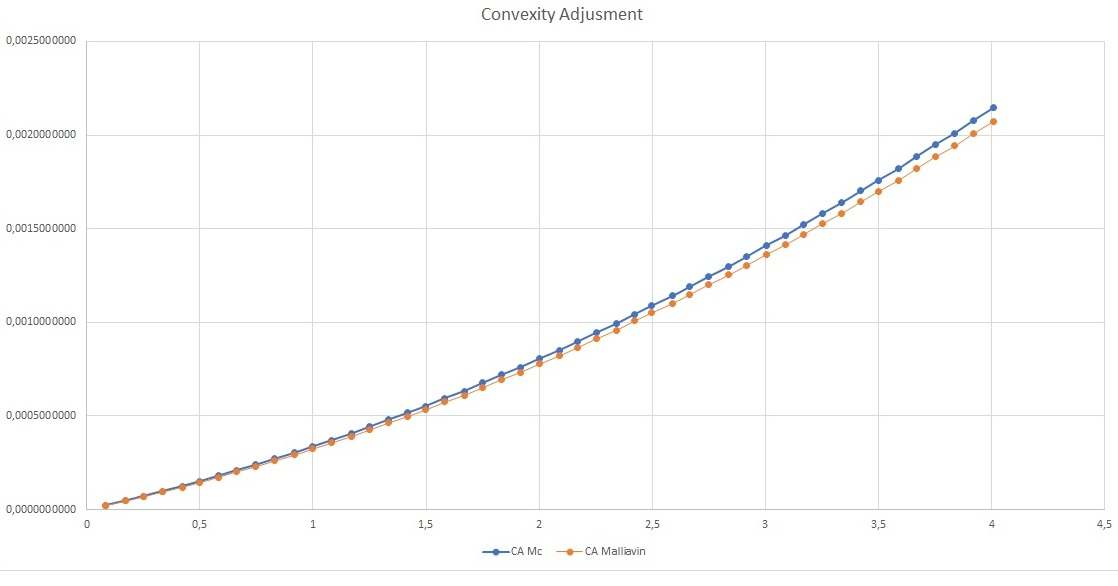
\includegraphics[scale=0.3]{Figures/future_convexity.jpg}
		\caption{Convexity Mc Vs Convexity Malliavin}
	\end{center}
\end{figure} 


\subsection{OIS futures}
In this we will derive the covexity adjustment for overnight-indexed swap (OIS) under. We will define for $t_0 < t_1$
\begin{align*}
R(t_0,t_1) &= \frac{\exp\left(\int_{t_0}^{t_1}r_{ois,u} du \right) - 1}{t_1 - t_0} \\
R_{avg}(t_0,t_1) &= \frac{\int_{t_0}^{t_1}r_{ois,u} du}{t_1 - t_0}.
\end{align*}
We must observe, that both $R(\cdot,t_0,t_1)$ and $R_{avg}(\cdot,t_0,t_1)$  are not predictible and they are only observable in $t_1$. However, since
$R(\cdot,t_0,t_1)$ and $R_{avg}(\cdot,t_0,t_1)$ are flows that will be payed in $t_1$, we can considerer the expected value under the measure $\mathbb{Q}$ that will observable during whole period $[t_0, t_1]$. Let us define the next $\mathbb{Q}$ martingales  
\begin{align*} 
\bar{R}(t,t_0,t_1) &= \mathbb{E}_t^{\mathbb{Q}}\left( R(t_0,t_1)  \right) \\
\bar{R}_{avg}(t,t_0,t_1) &= \mathbb{E}_t^{\mathbb{Q}}\left( R_{avg}(t_0,t_1)  \right).
\end{align*}
We must do several obeservations. The first observation is that, if we define $F(t,t_0,t_1) = \mathbb{E}^{\mathbb{Q}^{t_1}}\left( R(t_0,t_1)\right)$, then we have that
\begin{align*}
F(t,t_0,t_1)&= \frac{1}{P_{ois}(t,t_1)}  \mathbb{E}_{t}^{\mathbb{Q}}\left(\exp\left(-\int_{t}^{t_1} r_{ois,u} du \right) R(t_0,t_1) \right) = \frac{\frac{P_{ois}(t,t_0)}{P_{ois}(t,t_1)} - 1}{t_1 - t_0}, \quad t \in [0,t_0] \\
F(t,t_0,t_1)&= \frac{1}{P_{ois}(t,t_1)} \mathbb{E}_{t}^{\mathbb{Q}}\left(\exp\left(-\int_{t}^{t_1} r_{ois,u} du \right) R(t_0,t_1) \right) = \frac{1}{t_1 - t_0} \left(\frac{\left( \exp\left(\int_{t}^{t_1}r_{ois,u} du\right)\right)}{P_{ois}(t_0,t)}-1\right), \quad  t \in  [t_0, t_1].
\end{align*}
The can define the convexity adjustment for $ R(t_0,t_1)$ the next way
\begin{equation}\label{R_ois_ca}
CA_{ois}(t,t_0,t_1) = F(t,t_0,t_1) - \bar{R}(t,t_0,t_1) 
\end{equation}
The second observation, is that under the dyam we must do is that
\begin{equation}\label{R_ois_avg}
\mathbb{E}^{\mathbb{Q}}\left(R_{avg}(t_0,t_1) \right) = \mathbb{E}^{\mathbb{Q}}\left( \frac{\log\left(1+ \delta_{t_0,t_1} R(t_0,t_1) \right)}{\delta_{t_0,t_1}} \right)  
\end{equation}
In order to compute $\mathbb{E}^{\mathbb{Q}}\left(R(t_0,t_1\right)$, we will define
\begin{equation*}
I(t_0,t_1) = \int_{t_0}^{t_1} r_s ds
\end{equation*}
If we take $D_s$ on $I(t_0,t_1)$ we have that
\begin{equation*}
D_sI(t_0,t_1) = \int_{\max(s, t_{0})}^{t_1}  D_s x_u du 
\end{equation*}
Now, if $t < t_0$, then from (\ref{clark-okone}) and (\ref{approximation_spot_E_s_x_t}), we have that 
\begin{align}\label{apprx_I_t0_t1}
I(t_0,t_1) &= \mathbb{E}_t^{\mathbb{Q}}\left(I(t_0,t_1)\right) + \int_{t}^{t_1}\int_{\max(s, t_{0})}^{t_1}  \mathbb{E}_s^{\mathbb{Q}}\left(\beta(s,u,x_s,y_s) \bar{M}(s,u) \right) du dW_s^{\mathbb{Q}} \nonumber \\
&\approx \mathbb{E}_t^{\mathbb{Q}}\left(I(t_0,t_1)\right) + \int_{t}^{t_1}\int_{\max(s, t_{0})}^{t_1} \beta(s,u,x_0,\bar{y}_s) du dW_s^{\mathbb{Q}}\nonumber \\
&= \mathbb{E}_t^{\mathbb{Q}}\left(I(t_0,t_1)\right) + \int_{t}^{t_1} g(s)h(s,x_0,\bar{y}_s)\int_{\max(s, t_{0})}^{t_1} \exp\left( -\int_{s}^{u} k_{s^{\prime}} ds^{\prime}\right) du dW_s^{\mathbb{Q}}.
\end{align}
Then, using the previous approximation, we get that
\begin{align*}
1 + \delta_{t_0,t_1}\mathbb{E}_t^{\mathbb{Q}}\left(R(t_0,t_1)\right) &= \mathbb{E}_t^{\mathbb{Q}}\left( \exp(I(t_0,t_1)) \right)\\
&\approx \exp\left(\mathbb{E}_t^{\mathbb{Q}}\left(I(t_0,t_1)\right)\right)  \mathbb{E}^{\mathbb{Q}}\left(\exp\left(\int_{t}^{t_1} \Gamma(s,t_0,t_1)dW_s^{\mathbb{Q}}\right)\right)
\end{align*}
where $\Gamma(s,t_0,t_1)= g(s)h(s,x_0,y_0)\int_{\max(s, t_{0})}^{t_1} \exp\left( -\int_{s}^{u} k_{s^{\prime}} ds^{\prime}\right)du$. 
Therefore, we have that
\begin{equation}\label{representation_i_0_t}
1 + \delta_{t_0,t_1}\mathbb{E}^{\mathbb{Q}}\left(R(t_0,t_1)\right) \approx \exp\left(\mathbb{E}^{\mathbb{Q}}\left(I(t_0,t_1)\right)\right)\exp\left(-\int_{t}^{t_1}\frac{\Gamma^{2}(s,t_0,t_1)}{2} ds\right)
\end{equation}
Therefore

\hspace{2cm}
\fboxsep1em
\fbox{\parbox{335pt}
{
\begin{equation}\label{convexity_ois_future}
\mathbb{E}_t^{\mathbb{Q}}\left(R(t_0,t_1)\right) \approx \frac{\exp\left(\mathbb{E}_t^{\mathbb{Q}}\left(I(t_0,t_1)\right)\right)\exp\left(-\int_{t}^{t_1}\frac{\Gamma^{2}(s,t_0,t_1)}{2} ds\right) - 1}{\delta_{t_0,t_1}}
\end{equation}
}}
In order to get an approximation of $\mathbb{E}^{\mathbb{Q}}\left(R_{avg}(t_0,t_1)\right)$ with base $\mathbb{E}^{\mathbb{Q}}\left(R(t_0,t_1)\right)$, we must note that 
\begin{equation*}
\mathbb{E}_t^{\mathbb{Q}}\left(R_{avg}(t_0,t_1)\right) = \frac{\mathbb{E}_t^{\mathbb{Q}}\left( \log(1+ \delta_{t_0,t_1} R(t_0,t_1))\right)}{ \delta_{t_0,t_1}}.
\end{equation*}
Then from (\ref{representation_i_0_t}) we get that

\fboxsep1em
\fbox{\parbox{360pt}
{
\begin{equation}\label{convexity_avg_ois_future}
\mathbb{E}_t^{\mathbb{Q}}\left(R_{avg}(t_0,t_1)\right) = \frac{\mathbb{E}_t^{\mathbb{Q}}\left(I(t_0,t_1)\right) }{\delta_{t_0,t_1}} \approx \frac{\log\left(1+\delta_{t_0,t_1}  \mathbb{E}_t^{\mathbb{Q}}\left(R(t_0,t_1)\right) \right)}{\delta_{t_0,t_1}} - \frac{\int_{0}^{t_1}  \Gamma^{2}(s,t_0,t_1) ds}{2\delta_{t_0,t_1}}
\end{equation}
}}

\begin{remark}
We must observe that for the case $t_0 < t < t_1$ we can compute the convexity adjusment in a similar way when $t < t_0$, but in this case we have to define
\begin{equation*}
I(t,t_1)=\int_{t}^{t_1} r_s ds
\end{equation*}
and 
\begin{align*}
R(t_0,t_1) &= \frac{\frac{\exp(\int_{t}^{t_1} r_{ois,s} ds )}{P_{ois}(t_0,t)} - 1}{t_1 - t_0} \\
R_{avg}(t_0,t_1) &= \frac{\int_{t_0}^{t} r_{ois,s} ds}{t_1-t_0} +  \frac{\int_{t}^{t_1} r_{ois,s} ds}{t_1-t_0}.   
\end{align*}
\end{remark}

\begin{example}\label{example_convexity_hw_ois}
The same way that in the example (\ref{example_ca_future}), we will suppose a Hull-White model with constan mean reversion $k=0.003$ and volatility $\sigma=0.01$. It is easy to show in the case of the Hull-White model
\begin{align*}
\Gamma(s,t_0,t_1) &= \frac{\sigma \exp(-ks)}{k}\left(\exp(-k(\max(s,t_0) - s)) - \exp(-k(t_1-s))\right)\\
\mathbb{E}^{\mathbb{Q}}\left(I(t_0,t_1)\right)&=-\log\left(\frac{P_{ois}(0,t_1)}{P_{ois}(0,t_0)}\right) + \frac{\sigma^{2}}{2k^{2}}\left(\delta_{t_0,t_1} - 2 \frac{\exp(-kt_0) - \exp(-kt_1)}{k} + \frac{\exp(-2kt_0) - \exp(-2kt_1)}{2k}  \right).
\end{align*}
Therefore we have that
\begin{align*}
\frac{\int_{0}^{t_1} \Gamma^{2}(s,t_0,t_1) ds}{2} &= \frac{\sigma^{2}}{2k^2} \int_{0}^{t_1}  \exp(-2ks)\left(\exp(-k(\max(s,t_0) - s)) - \exp(-k(t_1 - s))\right)^{2} ds \\
&= \frac{\sigma^{2}}{2k^2} \int_{0}^{t_0} \exp(-2ks)\left(\exp(-k(t_0 - s)) - \exp(-k(t_1 - s))\right)^{2} ds\\
&+ \frac{\sigma^{2}}{2k^2} \int_{t_0}^{t_1} \exp(-2ks)\left(1 - \exp(-k(t_1 - s))\right)^{2} ds\\
&= \frac{\sigma^{2}t_0}{2k^{2}} \left( \exp(-kt_0) + \exp(-2kt_1) - 2 \exp(-k(t_1+t_0)) \right)\\  
&+ \frac{\sigma^{2}}{2k^{2}} \left(\frac{\exp(-2kt_0) - \exp(-2kt_1)}{2k}  + \exp(-kt0)t0 - 2 \frac{\exp(-2kt_0) - \exp(-k(t_0 + t_1))}{k}  \right)
\end{align*}(we have to review this integral).
Then, if we substitute the last equalities in (\ref{convexity_ois_future}) we get an approximation for OIS future at $t=0$. The next figure, show accuracy of (\ref{convexity_ois_future}) and (\ref{convexity_avg_ois_future}) for the particular case of a Hull-White model.


\begin{figure}
\begin{subfigure}{.5\textwidth}
  \centering
  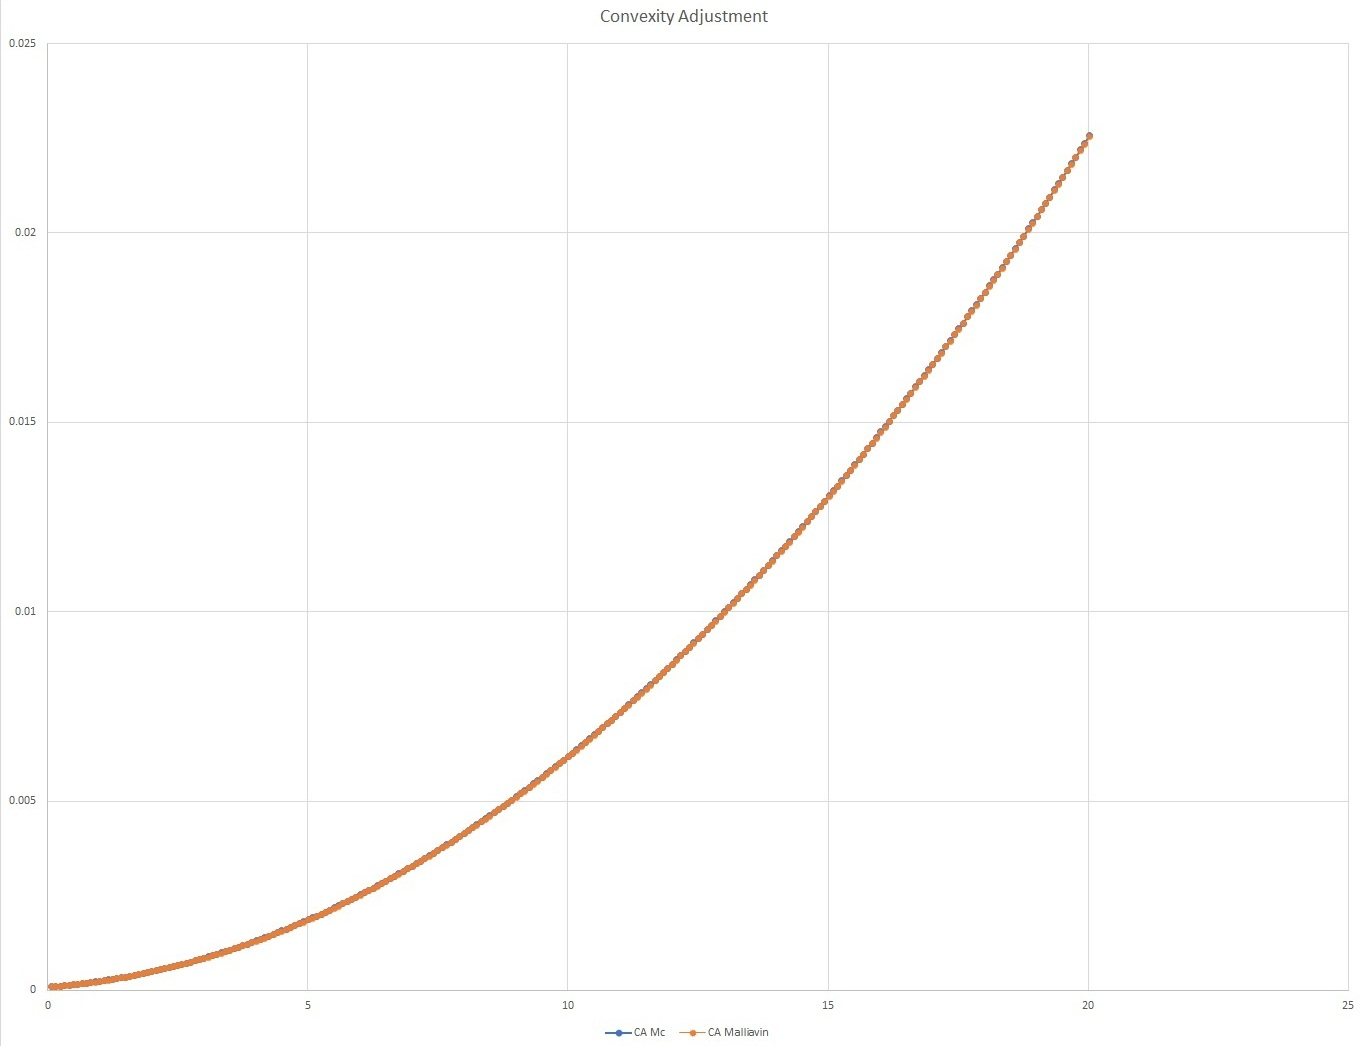
\includegraphics[scale=0.2]{Figures/convexity_ois.jpg}
		\caption{Convexity Mc Vs Convexity Malliavin}
\end{subfigure}
\begin{subfigure}{.5\textwidth}
  \centering
  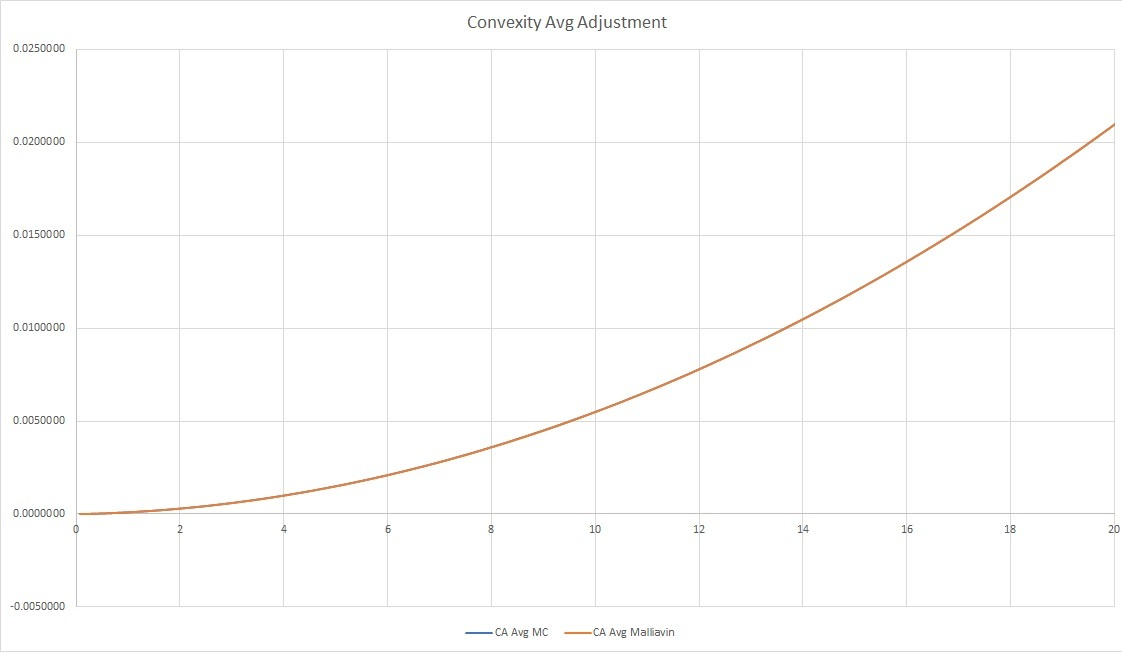
\includegraphics[scale=0.2]{Figures/convexity_avg_ois.jpg}
		\caption{Convexity Avg Mc Vs Convexity Avg Malliavin}
\end{subfigure}
\caption{Convexity adjustment for compounding and average OIS}
\end{figure} 
\end{example}

\newpage
\subsection{FRAs in arrears}
The price of a FRA in arrears, is the most classic example between the porducts with convexity adjustment. The cash flows associated to a FRAs in arrears is $L_{E}(t_1,t_1,t_2)$ in $t_1$. Therefore the payment will be
\begin{equation}
P_{E}(0,t_1)\mathbb{E}^{\mathbb{Q}^{t_1}}\left( L_{E}(t_1,t_1,t_2\right).
\end{equation}
The expected value is clearly taken with respect to the wrong martingale, because $L_{E}(t,t_1,t_2)$ is martingale under the measure $\mathbb{Q}^{t_2}$. In order to calculate, the convexity adjustment we will use as before Clark-Ocone to get a representation for $L_{E}(t_1,t_1,t_2)$ i.e
\begin{equation}\label{general_convexity_fras}
L_{E}(t_1,t_1,t_2) = \mathbb{E}^{\mathbb{Q}^{t_2}}\left(L_{E}(t_1,t_1,t_2) \right) + \int_{0}^{t_1} \mathbb{E}^{\mathbb{Q}^{t_2}}\left(D_s L_{E}(t_1,t_1,t_2) \right) dW^{\mathbb{Q}^{t_2}}_{s}
\end{equation}
The if we suppose the HJM dynamic (\ref{estimation_forward_rate_curve})and we take $\mathbb{E}^{^{\mathbb{Q}^{t_1}}}(\cdot)$ we get
\begin{align*}
\mathbb{E}^{\mathbb{Q}^{t_1}}\left(L_{E}(t_1,t_1,t_2) \right) &= L_{E}(0,t_1,t_2) + \mathbb{E}\left( \int_{0}^{t_1} \mathbb{E}^{\mathbb{Q}^{t_2}}\left(D_s L_{E}(t_1,t_1,t_2) \right) dW^{\mathbb{Q}^{t_2}}_{s}\right)\\
&= L_{E}(0,t_1,t_2) + \mathbb{E}\left( \int_{0}^{t_1} \mathbb{E}^{\mathbb{Q}^{t_2}}\left(D_s L_{E}(t_1,t_1,t_2) \right) (\nu(s,t_2)-\nu(s,t_1)) ds \right)
\end{align*}
Where we have used that 
\begin{equation*}
dW^{\mathbb{Q}^{t_2}}_s = dW^{\mathbb{Q}^{t_1}}_s + (\nu(s,t_2) - \nu(s,t_1)) ds 
\end{equation*}
Now from (\ref{approximation_D_s_x_t}) we have that 
\begin{equation*}
D_s L(t_1,t_1,t_2) = \frac{G(t_1,t_2)}{\delta_{t_1,t_2}P_{E}(t_1,t_2)} D_s x_{t_1} \approx \frac{G(t_1,t_2)}{\delta_{t_1,t_2}P_{E}(0,t_1,t_2)} \beta(s,t_1, x_0, \bar{y}_s)\bar{M}(s,t_1)
\end{equation*}
Therefore, if we define and we use (\ref{approsimation_E_s_x_t}) we have that
\begin{equation*}
CA(t_0,t_1) = \mathbb{E}^{\mathbb{Q}^{t_1}}\left( L_{E}\left(t_1,t_1,t_2\right)\right) - L_{E}\left(0,t_1,t_2\right)
\end{equation*}
and we use the last approximation and (\ref{general_convexity_fras}), we can get the next approximation for $CA(t_0,t_1)$ 
\hspace{2cm}
\fboxsep1em
\fbox{\parbox{475pt}
{
\begin{equation}\label{ca_approximations_fra_arrears}
CA(t_0,t_1) \approx  \frac{G(t_1,t_2)}{\delta_{t_1,t_2}P_{E}(0,t_1,t_2)} \int_{0}^{t_1} \beta(s,t_1, x_0, \bar{y}_s) \exp\left(-\int_{s}^{t_1} \partial_x \beta(u,t_1,x_0,y_0) \nu(u,t_2) du \right) (\nu(s,t_2) - \nu(s,t_1)) ds.
\end{equation}
}}
\begin{example}
To check how works the last approximation. We will restrict a Hull-White model with mean reversion and volatility constant. We will use are $\sigma=0.1$, $k=0.007$ for our model. The analytical approximation that we get from (\ref{ca_approximation_futures}) is
\begin{equation*}
CA(t_0,t_1) \approx \frac{G(t_1,t_2)}{\delta_{t_1,t_2}P_{E}(0,t_1,t_2)}  \frac{\sigma^{2}}{k} \int_{0}^{t_1} \exp(- k(t_1 + u)) -   \exp(- k(t_2 + u)) du 
\end{equation*}
We have checked the last approximation using MC method to compute the value of a FRA in arrears. We will show the result of the simulation in the next figure

\begin{figure}[h]
	\begin{center}
		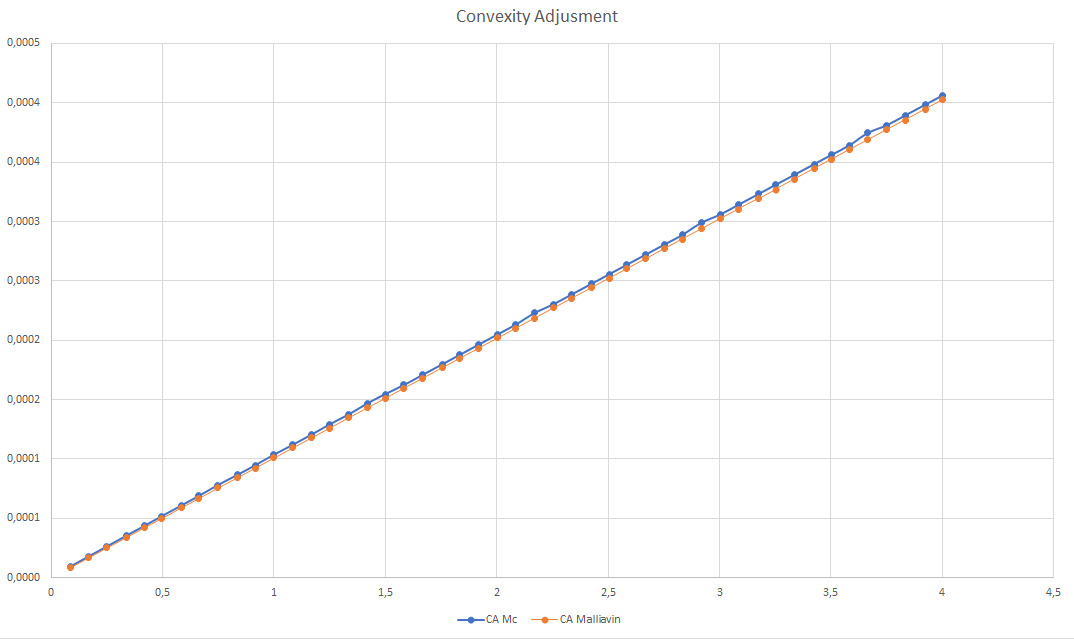
\includegraphics[scale=0.3]{Figures/fra_convexity.jpg}
		\caption{Convexity Mc Vs Convexity Malliavin}
	\end{center}
\end{figure} 
 
\end{example}

\subsection{CMSs}
In this last section we will study convexity adjustment for a CMS. Let us to introduce some notation, we will use it throughout the section. We will define the swap rate from $t_a$ to $T_b$ at time $t$
\begin{equation*}
S_{a,b}(t) = \frac{\sum_{i=1}^{n_E}\delta_{t^{E}_{i-1}, t^{E}_i} L^{E}(t,t^{E}_{i-1}, t^{E}_{i}) P_{ois}(t,t^{E}_{i})}{01(t,t_a,T_b)}
\end{equation*}
where
\begin{align*}
01(t,t_a,t_b) = \sum_{j=1}^{n_f} \delta_{t^{f}_{i-1}, t^{f}_i} P_{ois}(t,t^{f}_{j}) \\
t_a=t^{E}_0 < t^{E}_i< \cdots < t^{E}_{n_E}=t_b \quad i=0,\cdots,n_E&  \\
t_a=t^{f}_0 < t^{f}_j< \cdots < t^{f}_{n_f}=t_b \quad j=0,\cdots,n_f&
\end{align*}
The same way, we will define the OIS swap rate as
\begin{equation*}
S^{ois}_{a,b}(t) = \frac{P_{ois}(t,T^{E}_a) - P_{ois}(t,T^{E}_b)}{01(t,t_a,t_b)}. 
\end{equation*}

\begin{remark}
We must note that from (\ref{bond_forward})we have that
\begin{equation*}
S_{a,b}(t) = S^{ois}_{a,b}(t) + \frac{\sum_{i=1}^{n_E}\delta_{t^{E}_{i-1}, t^{E}_i} \alpha(t,t^{E}_{i-1}, t^{E}_{i}) P_{ois}(t,t^{E}_{i})} {01(t,t_a,t_b)}
\end{equation*}
where $ \alpha(t,t^{E}_{i-1}, t^{E}_{i})  = \frac{\frac{H(t,t^{E}_{i-1})}{H(t,t^{E}_{i})} - 1}{\delta_{t^{E}_{i-1}, t^{E}_i}}$. How we have a one-factor HJM model, we can suppose that variability of $\alpha(t,t^{E}_{i-1}, t^{E}_{i})$ is low, and therefore it is reasonable to freeze it at time $t=0$. Of this way, we have that
\begin{equation}\label{approximation_basis_swap}
S_{a,b}(t) \approx S^{ois}_{a,b}(t) + \frac{\sum_{i=1}^{n_E}\delta_{t^{E}_{i-1}, t^{E}_i} \alpha(0,t^{E}_{i-1}, t^{E}_{i}) P_{ois}(0,t^{E}_{i})} {01(0,t_a,t_b)}.
\end{equation}

\end{remark}

Now, we suppose that we have a flow in $t_a < t_p < t_b$ with value $S_{a,b}(t_a)$. We know that, $S_{a,b}(t_a)$ is a martingale under the measure $\mathbb{Q}^{01}$, but not under the measure $\mathbb{Q}^{t_p}$. Therefore, we we have to take into consideration the effect to compute the expected value of $S_{a,b}(t_a)$ in a measure which is not its natural measure. Then, the convexity adjustment for a CMS is
\begin{equation}
CA_{CMS}(t_p) = \mathbb{E}^{t_p}\left(S_{a,b}(t_a)\right) - S_{a,b}(0).
\end{equation} 
After some changes of measure, it is easy to show that
\begin{align}\label{expected_t_p_cms}
\mathbb{E}^{t_p}\left(S_{a,b}(t_a)\right) &= \frac{1}{M(0,t_p)} \mathbb{E}^{01}\left(S_{a,b}(t_a) M(t_a,t_p)\right) \nonumber \\
&= \frac{1}{M(0,t_p)} \mathbb{E}^{01}\left(S_{a,b}(t_a) \mathbb{E}^{01}\left( M(t_a,t_p)|S_{a,b}(t_a)\right) \right) \nonumber\\
\mathbb{E}^{t_p}\left(S_{a,b}(t_a)\right) &\approx  \frac{1}{M(0,t_p)} \mathbb{E}^{01}\left(S^{ois}_{a,b}(t_a) \mathbb{E}^{01}\left( M(t_a,t_p)|S_{a,b}(t_a)\right) \right) + \frac{\sum_{i=1}^{n_E}\delta_{t^{E}_{i-1}, t^{E}_i} \alpha(0,t^{E}_{i-1}, t^{E}_{i}) P_{ois}(0,t^{E}_{i})} {01(0,t_a,t_b)}
\end{align}
with $M(t,t_p)= \frac{P_{ois}(t,t_p)}{01(t,t_a,t_p)}$. From te previous expression, we must note that under assumption of not stochastic basis, we must to compute the convexity adjustment for the OIS swap rate. Another, complicated point, is the expected value 
$$
\mathbb{E}^{01}\left( M(t_a,t_p)|S_{a,b}(t_a)\right).
$$
In order to reduce this complexity, it is a common practice to assume that $M(t_a,t_p)$ is a funtion of the swap rate $S_{a,b}(t_a)$ i.e   $M(t_a,t_p)=f(S_{a,b}(t_a))$, of this way the last expected value is trivial. The function $f(\cdot)$ is known as mapping function, and there is a vast literatura about how to choose it (see Piterbarg Volumen III, Hagan paper convexity withour replication). We will, try to do an approach, without to specify any mapping function. If we apply Clark-Ocone formula to $M(t_a,t_p)$ we get that
\begin{equation} \label{clark_ocone_swap_m}
M(t_a,t_p) = M(0,t_p)+ \int_{0}^{t_a} \mathbb{E}_s^{01}\left(D_s M(t_a,t_p)\right) dW^{01}_s
\end{equation}
Then, if we sustitute the last expressions in (\ref{expected_t_p_cms}) we have that
\begin{align}\label{cms_first_order_convexity}
\mathbb{E}^{t_p}\left(S_{a,b}(t_a)\right) =& S^{ois}_{a,b}(0) + \frac{1}{M(0,t_p)} \mathbb{E}^{01}\left( S^{ois}_a,b(t_a) \int_{0}^{t_a} \mathbb{E}^{0,1}_s\left(D_sX_{t_a}\partial_x M(t_a,t_p)  \right) dW^{0,1}_s   \right) \nonumber \\
=&  S^{ois}_{a,b}(0) + \frac{1}{M(0,t_p)} \mathbb{E}^{01}\left(\int_{0}^{t_a} D_s X_{t_a} \partial_x S_{a,b}(t_a) \mathbb{E}^{0,1}_s\left(D_sX_{t_a}\partial_x M(t_a,t_p)  \right) ds   \right) \nonumber \\
\approx&  S^{ois}_{a,b}(0) + \frac{\partial_x S^{ois}_{a,b}(t_a, \bar{x}_0(t_a),\bar{y}(t_a))\partial_x M(t_a,t_p, \bar{x}_0(t_a),\bar{y}(t_a))}{M(0,t_p)} \mathbb{E}^{0,1}\left( \int_{0}^{t_a} \left(\mathbb{E}_s^{0,1}\left( D_s x_{t_a}\right)\right)^{2} ds  \right)
\end{align}

\begin{remark}
We must observe that, if we want to use the last approximation  we must be able to approximate $\mathbb{E}_s^{0,1}\left( D_s x_{t_a}\right)$. The simplest case, if when $\eta(t,x_t,y_t) \eta(t)$ as for example happens in the Hull-White model or Ho-Lee model. The general case, has been treated in (\ref{approximation_under_annuity_measeure_d_s}). 
\end{remark}

\begin{example}
In order to check the accuracy of the last approximation, we will compute with Monte Carlo method the exact value of $\mathbb{E}^{t_p}\left(S^{ois}_{a,b}(t_a)\right)$ under spot measure $\mathbb{Q}$ i.e we will compute  $\frac{1}{P(0,t_p)}  \mathbb{E}^{\mathbb{Q}}\left(\frac{S_{a,b}(t_a)}{\beta_{t_a}} \right)$. In the case of a Hull-White model, we have that
$$
D_s x_{t_a} = \sigma \exp(-(t_a - s))
$$
therefore (\ref{cms_first_order_convexity}) is equal to
\begin{equation*}
\mathbb{E}^{t_p}\left(S_{a,b}(t_a)\right) \approx  S^{ois}_{a,b}(0) + \frac{\partial_x S^{ois}_{a,b}(t_a, \bar{x}_0(t_a),\bar{y}(t_a))\partial_x M(t_a,t_p, \bar{x}_0(t_a),\bar{y}(t_a))}{M(0,t_p)} \frac{\sigma^{2}(1-\exp(-2kt_a))}{2k}.
\end{equation*}
In the next figure, we can see the convexity adjustment for a CMS where the tenor of the underlying swap is 5Y using the last approximation and Montecarlo method with parameters for the Hull-White model $\sigma=0.01$ and $k=0.0007$

\begin{figure}[h]
	\begin{center}
		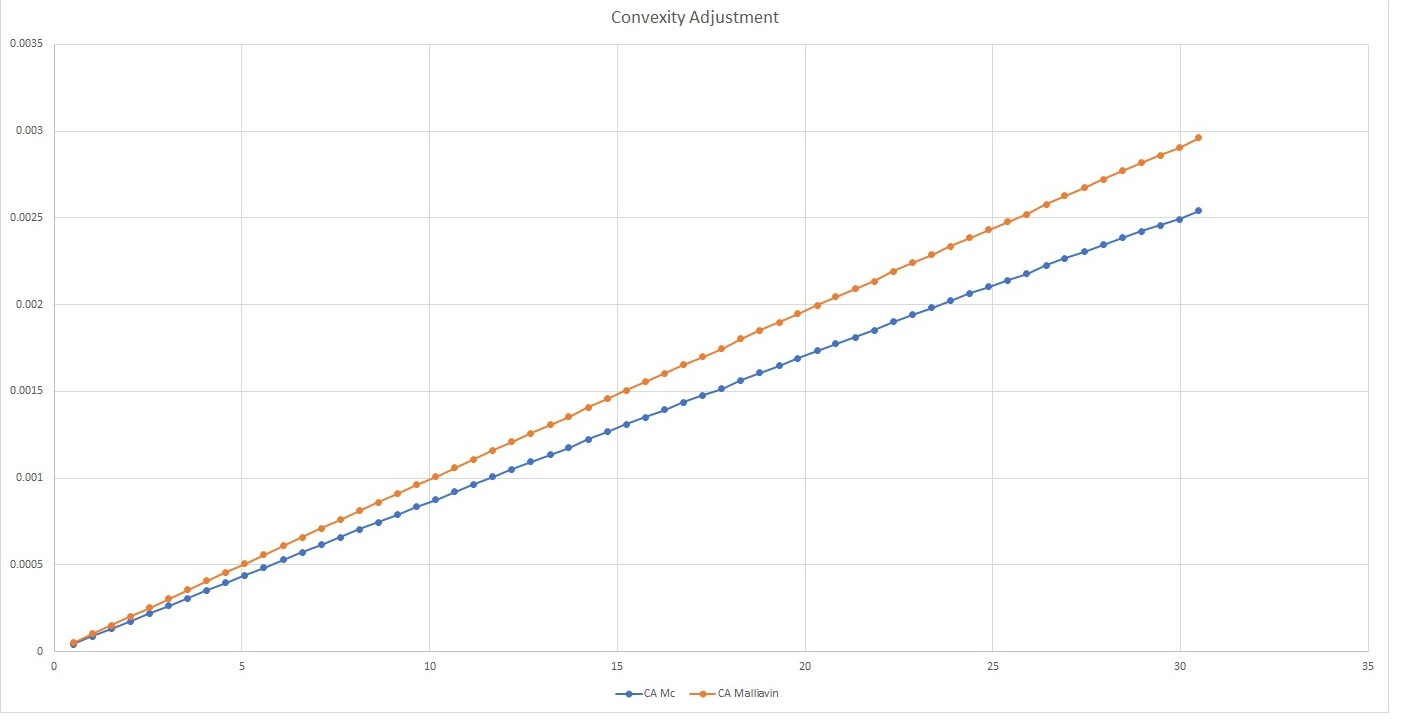
\includegraphics[scale=0.25]{Figures/cms_convexity_order.jpg}
		\caption{Convexity Mc Vs Convexity Malliavin}
	\end{center}
\end{figure} 
\end{example}

\section{Conclusions}\label{sec:Conclusion}



\section*{Appendix}
\appendix
\renewcommand{\thesection}{\Alph{section}.\arabic{section}}



\section{Approximation of $\mathbb{E}_s^{t_p}\left(D_s x_{t_a}\right)$}
\label{expected_forward_measure_malliavin_derivative_x_t}
From (\ref{short_rate_cheyette}) is easy to show that
\begin{equation*}
x_{t_a} = \int_{0}^{t_a} \exp\left(-\int_{s}^{t_a}k_u du\right) y_u du + \int_{0}^{t_a}  \exp\left(-\int_{s}^{t_a}k_u du \right) \eta(u,x_u,y_u) dW_u^{\mathbb{Q}}  
\end{equation*}
In order to get an approximation for $D_sX_{t_a}$ we must to avoid the recurrence in the Malliavin derivative of $X_{t_a}$. Follow, the ideas of Piterbarg Volume II, we can approximate $y_t$ the next way
\begin{equation*}
y_t \approx \int_{0}^{t} \exp\left(-2\int_{u}^{t} k_{u^{\prime}} du^{\prime} \right) \eta^{2}(u,x_0,y_0) du
\end{equation*}
Therefore, if we define $\bar{y}(t)= \int_{0}^{s} \exp\left(-2\int_{u}^{s} k_{u^{\prime}} du^{\prime} \right) \eta(u,x_0,y_0)$, we have that
\begin{equation}\label{approximation_x_t_a}
X_{t_a} \approx \bar{X}(t_a):= \bar{x}_0(t_a)  + \int_{0}^{t_a} \exp\left(-\int_{s}^{t_a}k_u du\right) \bar{y}(u) du + \int_{0}^{t_a}  \exp\left(-\int_{s}^{t_a}k_u du \right) \eta(u,\bar{x}(u),\bar{y}(u)) dW_u^{\mathbb{Q}}  
\end{equation}
With initial condition  $\bar{x}_{0}(t_a)$ is such that $S_{a,b}(t_a,\bar{x}_0(t_a), \bar{y}_{t_a}) = S_{a,b}(0)$ (see Piterbarg Volume II). Now, we must remember that 
\begin{equation*}
dW^{\mathbb{Q}^{t_p}} = dW^{\mathbb{Q}} + \bar{\nu}(t,t_p) dt 
\end{equation*}
where $\bar{\nu}(t,t_p) = \int_{t}^{t_p} \eta(s,\bar{x}_s,\bar{y}_s) ds $. Then, we have the next approximation of $\bar{x}_{t_a}$ under measure $\mathbb{Q}^{t_p}$
\begin{align*}
X_{t_a} &\approx \bar{x}_0  + \int_{0}^{t_a} \exp\left(-\int_{s}^{t_a}k_u du\right) \bar{y}_s ds - \int_{0}^{t_a} \exp\left(-\int_{s}^{t_a}k_u du\right) \bar{\nu}(s, t_p) \eta(s,\bar{x}_s,\bar{y}_s) ds +  \\
&+ \int_{0}^{t_a}  \exp\left(-\int_{s}^{t_a}k_u du \right)\eta(s,\bar{x}_s,\bar{y}_s) dW_s^{\mathbb{Q}^{t_p}}  
\end{align*} 
Then, if we take $D_s$ on $\bar{X}_{t_a}$ we get that (esto hay que formalizarlo...)
\begin{equation}\label{approximation_D_s_x_t}
D_sX_{t_a} \approx  \exp\left(-\int_{s}^{t_a}k_u du \right) \eta(s,\bar{x}_0(t_a),\bar{y}(t_a))\bar{M}(s,t_a)
\end{equation}
where
\begin{align*}
\bar{M}(s,t_a) &= \exp\left(-\int_{s}^{t_a} \left( \frac{\left(\partial_x \beta(u,t_a,\bar{x}_0,\bar{y}_{t_a})\right)^{2}}{2} - \exp\left(-\int_{u}^{t_a}k_u du\right) \partial_x (\eta(u, \bar{x}_u, \bar{y}_{u}) \bar{\nu}(u,t_p))\right) du \right) \\ 
&\cdot\exp\left(\int_{s}^{t_0} \partial_x \beta(u,t_a,\bar{x}_0,\bar{y}_{t_a}) dW^{\mathbb{Q}}_u \right)
\end{align*}
With $\beta(u,t_a,x,y) = \exp\left(-\int_{u}^{t_a}k_u^{\prime} du^{\prime}\right) \partial_x \eta(u,x,y)$. Therefore, from previous equalities, we have that

\begin{equation}\label{approsimation_E_s_x_t}
\mathbb{E}_s^{t_p}\left(D_s x_{t_a}\right) \approx \eta(s,\bar{x}_0(s),\bar{y}_s) \exp\left(-\int_{s}^{t_a}k_u du \right) \exp\left(-\int_{s}^{t_a} \exp\left(-\int_{u}^{t_a}k_u du\right)\partial_x (\eta(u, \bar{x}_u, \bar{y}_{u}) \bar{\nu}(u,t_p)) du \right).
\end{equation}

\section{Approximation of $\mathbb{E}_s^{\mathbb{Q}}\left(D_s x_{t_a}\right)$}
Following the same procedure as before, we have that
\begin{equation*}
X_{t_a} \approx \bar{X}(T_a):= \bar{x}_0(t_a)  + \int_{0}^{t_a} \exp\left(-\int_{s}^{t_a}k_u du\right) \bar{y}(u) du + \int_{0}^{t_a}  \exp\left(-\int_{s}^{t_a}k_u du \right) \eta(u,\bar{x}(u),\bar{y}(u)) dW_u^{\mathbb{Q}}  
\end{equation*}
and therefore (see (\ref{approsimation_E_s_x_t}))
\begin{equation}
D_sX_{t_a} \approx  \exp\left(-\int_{s}^{t_a}k_u du \right) \eta(s,\bar{x}_0(t_a),\bar{y}_{T_a})\bar{M}(s,t_a)
\end{equation}
Now, if we take $\mathbb{E}^{\mathbb{Q}}\left(\cdot\right)$ we get
\begin{equation}\label{approximation_spot_E_s_x_t}
\mathbb{E}^{\mathbb{Q}}_s\left(D_sX_{t_a} \right) \approx \exp\left(-\int_{s}^{t_a}k_u du \right) \eta(s,\bar{x}_0(t_a),\bar{y}_{t_a})
\end{equation} 

\section{Approximation of $\mathbb{E}^{01}\left(x_{t_a}\right)$}
It is easy to show that the dynamic of the bond under HJM assumption is
\begin{equation}
\frac{dP(t,T)}{P(t,T)} = r_t dt - \nu(t,T)dW^{\mathbb{Q}}_t.  
\end{equation}
Therefore, if we apply Itô formula we have that 
\begin{equation}\label{annuity_spot_dynamic}
\frac{d01(t,t_a,t_b)}{01(t,t_a,t_b)} = r_t dt - \sigma_{01}(t,t_a,t_b)dW^{\mathbb{Q}}_t
\end{equation}
where 
\begin{equation} \label{annuity_vol}
\sigma_{01}(t,t_a,t_b) = \frac{\sum_{i=a+1}^{b} \delta_{i-1,i} P(t,t_i) \nu(t,t_i)}{01(t,t_a,t_b)}.
\end{equation}
From (\ref{annuity_vol}) and since $\frac{P_{ois}(t,T)}{01(t)}$ is a martingale, we have that
\begin{equation*}
dW^{01}_t = dW^{\mathbb{Q}}_t - \sigma_{01}(t,t_a,t_b)dt. 
\end{equation*}
Thwn can do the next approximation of (\ref{annuity_vol})
\begin{equation} \label{approximation_o1_vol}
\bar{\sigma}_{01}(t,t_a,t_b) \approx \sum_{i=a+1}^{b} w_i \nu(t,t_i,x_0,y_0)
\end{equation}
with $w_i=\frac{\delta_{i-1,i} P(0,T_i)}{01(0,t_a,t_b)}$. Now, if we use (\ref{short_rate_cheyette}) and the previous approximation we have that
\begin{align}
x_{t_a} &\approx \bar{x}_0(t_a)  + \int_{0}^{t_a} \exp\left(-\int_{s}^{t}k_u du\right) \bar{y}(u) du + \int_{0}^{t_a}  \exp\left(-\int_{s}^{t_a}k_u du \right) \eta(u,\bar{x}(u),\bar{y}(u)) dW_u^{\mathbb{Q}} \nonumber \\
&=  \bar{x}_0(t)  + \int_{0}^{t_a} \exp\left(-\int_{s}^{t_a}k_u du\right) \bar{y}(u) du + \int_{0}^{t_a} \exp\left(-\int_{s}^{t_A}k_u du \right) \eta(u,\bar{x}(u),\bar{y}(u)) \bar{\sigma}_{01}(u, T_a, T_b) du  + \nonumber \\ 
& \int_{0}^{t_a} \exp\left(-\int_{s}^{t_a}k_u du \right) \eta(u,\bar{x}(u),\bar{y}(u)) dW_u^{01} 
\end{align}
Therefore, we have that
\begin{align}
\mathbb{E}^{01}\left(x_t\right) &\approx \bar{x}_0(t_a)  + \int_{0}^{t_a} \exp\left(-\int_{s}^{t_a}k_u du\right) \bar{y}(u) du \nonumber \\ 
+ &\int_{0}^{t_a} \exp\left(-\int_{s}^{t_a}k_u du \right) \eta(u,\bar{x}(u),\bar{y}(u)) \bar{\sigma}_{01}(u, t_a, t_b) du
\end{align}

\section{Approximation of $\mathbb{E}^{01}\left(D_s x_{t_a} \right)$}\label{approximation_under_annuity_measeure_d_s}
Let us to remember that $\nu(t,t_i)=h(t,x_t,y_t) \frac{G(t,t_i)}{\beta_{t,k}}$ with  $\beta_{t,k} = \exp\left(\int_{0}^{t}k(u)\right)$. Then, we can do the next approximation 
$$
\nu(t,t_i) \approx \nu(t,t_i, \bar{x}_t, \bar{y}_t),
$$ 
therefore 
\begin{equation*}
D_s \nu(t,T_i) \approx  \partial_x \nu(t,T_i, \bar{x}_t, \bar{y}_t) D_s \bar{x}_t  \frac{G(t,t_i)}{\beta_{t,k}}
\end{equation*}
A cosequence of the last approximation is that 
\begin{equation}
D_s \sigma_{0,1}(t,t_a,t_b) \approx  D_s \bar{x}_t \mu(t,t_a,t_b)
\end{equation}
where 
$$
\mu(t,T_a,T_b) =  \sum_{i=a+1}^{b} w_i \partial_x \nu(t,t_i, \bar{x}_t, \bar{y}_t) \frac{G(t,t_i)}{\beta_{t,k}}.
$$
Now, if we use the last approximation and (\ref{approximation_o1_vol}) in (\ref{approximation_x_t_a}) together with the Girsanov's theorem, we have that
\begin{align*}
\bar{x}_{T_a} &\approx  \bar{x}_0(t_a)  + \int_{0}^{t_a} \exp\left(-\int_{s}^{t_a}k_u du\right) \bar{y}(u) du + \int_{0}^{t_a} \exp\left(-\int_{s}^{t_a}k_u du\right) \bar{\sigma}_{01}(u,t_a,t_b) du \nonumber \\\
&+  \int_{0}^{t_a}  \exp\left(-\int_{s}^{t_a}k_u du \right) \eta(u,\bar{x}(u),\bar{y}(u)) dW_u^{\mathbb{Q}^{01}}.
\end{align*}
Therefore
\begin{equation*}
D_s \bar{x}_{t_a} \approx  \exp\left(-\int_{s}^{t_a}k_u du \right) \eta(s,\bar{x}_0,\bar{y}_{t_a})\bar{M}^{01}(s,t_a)
\end{equation*}
where
\begin{align*}
\bar{M}^{01}(s,t_a) &= \exp\left(-\int_{s}^{t_a} \left(\frac{\left(\partial_x \beta(u,T_a,\bar{x}_0,\bar{y}_{t_a})\right)^{2}}{2} + \exp\left(-\int_{u}^{t_a}k_u du\right)\eta(u,\bar{x}(u),\bar{y}(u) \mu(u,t_a,t_b) du \right)\right) \\
&\exp\left(\int_{s}^{t_a} \partial_x \beta(u,t_a,\bar{x}_0,\bar{y}_{t_a}) dW^{\mathbb{Q}^{01}}_u \right)
\end{align*}
and $\beta(u,t_a,x,y) = \exp\left(-\int_{u}^{t_a}k_u du\right) \partial_x \eta(u,x,y)$. Therefore

\begin{equation}\label{approximation_E_01_s_x_t}
\mathbb{E}^{01}_s\left(D_s x_{t_a}\right) \approx \eta(s,\bar{x_0(s)},\bar{y}_{s}) \exp\left(-\int_{s}^{t_a}k_u du \right) \exp\left(-\int_{s}^{t_a} \exp\left(\int_{u}^{t_a}k_u du\right)\eta(u,\bar{x}(u),\bar{y}(u) \mu(u,t_a,t_b) du \right).
\end{equation}

\section{Order of the approximation $\bar{x}_t$}
From (\ref{short_rate_cheyette}) is easy to show that
\begin{equation*}
x_{t_a} = \int_{0}^{t_a} \exp\left(-\int_{u}^{t_a}k_u du^{\prime}\right) G(u,t_a) \eta^{2}(u,x_u,y_u) du + \int_{0}^{t_a}  \exp\left(-\int_{u}^{t_a}k_u^{\prime} du \right) \eta(u,x_u,y_u) dW_u^{\mathbb{Q}} 
\end{equation*}
Therefore, we have that
\begin{align*}
(x_{t_a} - \bar{x}_{t_a})^2 &\leq 2 \left(\int_{0}^{t_a} \exp\left(-\int_{u}^{t_a}k_u^{\prime} du^{\prime}\right) G(u,t_a) (\eta^{2}(u,x_u,y_u) - \eta^{2}(u,x_0,y_0)) du \right)^{2} \\ 
&+ 2 \left(\int_{0}^{t_a}  \exp\left(-\int_{s}^{t_a}k_u^{\prime} du^{\prime} \right) (\eta(u,x_u,y_u)-\eta(u,\bar{x}_u,\bar{y}_u)) dW_u^{\mathbb{Q}}\right)^{2}
\end{align*}
Now, we will bound each integral term. We will call to the first term $(A)$ and the second $(B)$. From the hypothesis (\ref{boundedness_volatility}) we have that 
\begin{align*}
(A) &\leq 8 t_a \alpha^{2}_2 C^{2}_{x,y} \int_{0}^{t_a} \exp\left(-2\int_{u}^{t_a}k_u^{\prime} du^{\prime}\right) G^{2}(u,t_a) \|(x_u -x_0,y_u-y_0)\|^{2} du \\
&\leq 16 t_a \alpha^{2}_2 C^{2}_{x,y} \int_{0}^{t_a} \exp\left(-2\int_{u}^{t_a}k_u^{\prime} du^{\prime}\right) G^{2}(u,t_a) \|(x_u - \bar{x}_u,y_u-\bar{y}_u)\|^{2} du \\
&+ 16 t_a \alpha^{2}_2 C^{2}_{x,y} \int_{0}^{t_a} \exp\left(-2\int_{u}^{t_a}k_u^{\prime} du^{\prime}\right) G^{2}(u,t_a) \|(\bar{x}_u - x_0,\bar{y}_u-y_0)\|^{2} du
\end{align*}
and we take $\mathbb{E}^{\mathbb{Q}}\left(\cdot\right)$ on above inequality
\begin{align*}
\mathbb{E}^{\mathbb{Q}}\left((A)\right) &\leq 16  t_a \alpha^{2}_2 C^{2}_{x,y} \int_{0}^{t_a} \exp\left(-2\int_{u}^{t_a}k_u^{\prime} du^{\prime}\right) G^{2}(u,t_a) \mathbb{E}^{\mathbb{Q}}\left(\|(\bar{x}_u -x_0,\bar{y}_u-y_0)\|^{2}\right) du \\
&+\leq 16  t_a \alpha^{2}_2 C^{2}_{x,y} \int_{0}^{t_a} \exp\left(-2\int_{u}^{t_a}k_u^{\prime} du^{\prime}\right) G^{2}(u,t_a) \mathbb{E}^{\mathbb{Q}}\left(\|(x_u - \bar{x}_u,y_u-\bar{y}_u)\|^{2}\right) du
\end{align*}
Again, from the hypotheses (\ref{boundedness_volatility}) and (\ref{boundedness_reversion}) we can show that 
\begin{equation*}
\mathbb{E}^{\mathbb{Q}}\left(\|(\bar{x}_u -x_0,\bar{y}_u-y_0)\|^{2}\right) \sim \mathcal{O}(I(0,u,2))
\end{equation*}
In order to bound $(B)$, we will use the Doob's inequality and (\ref{boundedness_volatility}). Then
\begin{align*}
\mathbb{E}^{\mathbb{Q}}&\left((B)\right) \leq 2K \int_{0}^{t_a}  \exp\left(-2\int_{u}^{t_a}k_u^{\prime} du^{\prime} \right) (\eta(u,x_u,y_u)-\eta(u,\bar{x}_u,\bar{y}_u))^{2} du \\
& \leq 2K C^{2}_{x,y} \int_{0}^{t_a}  \exp\left(-2\int_{u}^{t_a}k_u^{\prime} du^{\prime} \right) \mathbb{E}^{\mathbb{Q}}\left(\|(x_u - \bar{x}_u, y_u - \bar{y}_u) \|^{2}\right) du
\end{align*}
On other hand, we have that
\begin{equation*}
\mathbb{E}^{\mathbb{Q}}\left((y_{t_a} - \bar{y}_{t_a})^{2} \right) \leq 4 \alpha^{2}_{2} C^{2}_{x,y} \int_{0}^{t_a} \exp\left(-2\int_{u}^{t_a}k_u^{\prime} du^{\prime}\right)\mathbb{E}^{\mathbb{Q}}\left(\|(x_u-\bar{x}_u,y_u-\bar{y}_u)\|^{2}\right) du    
\end{equation*}
Now, if we put all of the above together, we get that
\begin{equation*}
\mathbb{E}^{\mathbb{Q}}\left(\|(x_{t_a} - \bar{x}_{t_a},y_{t_a} - \bar{y}_{t_a})\|^{2}\right) \leq C_1H(t_a) + C_2\int_{0}^{t_a} \exp\left(-2\int_{u}^{t_a}k_u^{\prime} du^{\prime} \right) \mathbb{E}^{\mathbb{Q}}\left(\|(x_{u} - \bar{x}_{u},y_{u} - \bar{y}_{u})\|^{2}\right) du
\end{equation*}
where $C_1$ and $C_1$ are adequate positive constants and $H(t_a) \sim \mathcal{O}(\int_{0}^{t_a} I(0,u,2) du)$. To end, if we apply a slightly modified version of the Gronwall's lemma we have that
\begin{equation*}
\mathbb{E}^{\mathbb{Q}}\left(\|(x_{t_a} - \bar{x}_{t_a},y_{t_a} - \bar{y}_{t_a})\|^{2}\right) \leq C_1 H(t_a)+ \int_{0}^{t_a} \exp\left(- C_2 \int_{u}^{t} k(s^{\prime})  ds^{\prime} \right) H(u) du.
\end{equation*}

\newpage

% TODO: Change bibliographystyle according to the journal style - it should know the online entry, see Matsuda04
\bibliography{references/references, references/references-books,references/references-own,references/references-online}
%\bibliography{references-export}

\end{document}

